\documentclass[aspectratio=43]{beamer}

\usepackage[T1]{fontenc}
\usepackage[utf8x]{inputenc}
\usepackage[ngerman]{babel}
\usepackage{amsfonts,amsmath,amssymb,amsthm}
\usepackage{csquotes}

\usepackage{hyperref}

\usetheme[komms=false]{fbmathematik}

%%%%%%%%%%%%%%%%%%%%%%%%%%%%%%%%%%%%%%%%%%%%%%%%%%%%%%%%%%%
% Schriftfarben:
% tuklblau, tuklrot, warmgrau, kaltgrau;
% abgeschwächte Töne für die obigen Farben und schwarz:
% z.B. tuklblau7 für 70% tuklblau, warmgrau2 für 20%
% warmgrau oder schwarz6 für 60% schwarz,
% jeweils in den Schritten 10%, 20%, 40%, 60%, 70%, 80%;
% violette Schriftfarbe (Felix-Klein) hat den Namen fkz1
% hellviolette FKZ-Variante hat den Namen fkz2;
% KOMMS: kommsblau, kommsgruen, kommsgrau, kommsblaugrau
%%%%%%%%%%%%%%%%%%%%%%%%%%%%%%%%%%%%%%%%%%%%%%%%%%%%%%%%%%%



\title{Immer der Sonn' entgegen}
\subtitle{2. Zwischenbericht}
\author{Dominik Bendle \and Melissa Hasel \and Thomas Hofmann}
\date{\today}
\institute{TU Kaiserslautern}

\begin{document}

\begin{frame}[plain]

    % Leerzeilen vor und nach Titel sind offenbar nötig
    \Titel{logo}

\end{frame}

\begin{frame}
    \frametitle{Einbau von Höhendaten}
    Erster Versuch der Verfeinerung unseres Modells
    \begin{itemize}
        \item Betrachten von Höhendaten für besuchte Koordinaten
        \item[]$\rightarrow$ Jeweils mittlere Steigung
        \item[]$\rightarrow$ Einbezug der Geschwindigkeitsunterschiede
        \item Verwenden frei verfügbare SRTM-Daten (Shuttle Radar Topology Mission) der NASA
        \item[]$\rightarrow$ Zuordnung Koordinate--Höhe auf 30--90\,m genau
        \item[]$\rightarrow$ vorgefertigtes Matlab-Skript
        \item Daten verfügbar zwischen 59°\,S und 60°\,N.
    \end{itemize}
\end{frame}

\begin{frame}
    \frametitle{Geschwindigkeitsmodell}
    \begin{itemize}
        \item Verwenden einfaches Geschwindigkeitssmodell, um Laufgeschwindigkeit in
            Abhängigkeit von Steigung zu bestimmen
        \item Tobler's hiking function liefert Formel
            \begin{equation*}
                v = 6e^{-3{,}5 \left| \frac{d h}{d x} + 0{,}05\right|}
            \end{equation*}
            wobei $v$ die Geschwindigkeit, $dh$ der Höhenunterschied und $dx$ die
            vertikal zurückgelegte Distanz sind
    \end{itemize}
\end{frame}

\begin{frame}
    \frametitle{\enquote{Toblers Wanderfunktion}}
    \begin{figure}[t]
        \centering
        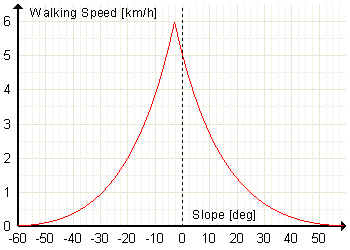
\includegraphics[width=0.70\textwidth]{bilder/thf.png}
        \caption{Werte in Abhängigkeit vom Steigungswinkel (Quelle: Wikimedia)}
    \end{figure}
\end{frame}

\begin{frame}
    \frametitle{Live-Plot}
    \centering
    \pause
    Einbeziehen der Daten hat letztendlich einen eher geringen Effekt auf die Laufbahn.
\end{frame}

\begin{frame}
    \frametitle{Interaktion mit OpenStreetMap}
    \begin{itemize}
        \item wollen Modell nun um reale Daten erweitern
        \item wählten OpenStreetMap als Provider für Daten
        \item[]$\rightarrow$ unbeschränkter Zugriff auf offene Daten
        \item 1. Idee: ausreichend großen, die Route umfassenden Bereich im Voraus laden
        \item[]$\rightarrow$ Problem: Matlab scheitert aus Speichergründen bereits am
            Laden von Karten der Größe Berlins, benötigen aber weitaus mehr Platz
        \item Lösung: Laden kontinuierlich kleine Kartenausschnitte (Karten der Größe
            100--500\,KB)
        \item Betrachten mit \enquote{highway}-Tag nur Straßen und Wege
    \end{itemize}
\end{frame}

\begin{frame}
    \frametitle{Arbeiten mit OpenStreetMap-Daten}
    \begin{itemize}
        \item verwenden opentreetmapfunctions, um OSM-XML in Matlab-Struct zu speichern
        \item[]$\rightarrow$ Verkehrsnetz in Adjazenzmatrix des ungerichteten Graphen
            dargestellt
        \item[]$\rightarrow$ Nachbarn eines Knoten leicht bestimmbar: zwei
            Verhaltensweisen:
            \begin{itemize}
                \item Knoten hat zwei Nachbarn: merken uns Vorgänger und wählen
                    Nicht-Vorgänger als nächsten Knoten
                \item[]$\rightarrow$ gehen bis zur nächsten Kreuzung, ohne umzudrehen
                \item sonst betrachte Richtungsvektoren zu allen Nachbaren (im $\mathbb
                    R^3$), bestimme optimale Gangrichtung, wähle optimalen Nachbarn mit
                    Skalarprodukt
                \item[]$\rightarrow$ falls alle Produkte $<0$, liegt Sonne bei jeder
                    Bewegung im Rücken, tue also nichts
            \end{itemize}
    \end{itemize}
\end{frame}

\end{document}
